\documentclass[tikz,border=8pt]{standalone}
\usepackage{tikz}
\usepackage{tkz-euclide}
\usepackage{amsmath, amssymb}

\usetikzlibrary{angles, quotes}

\begin{document}

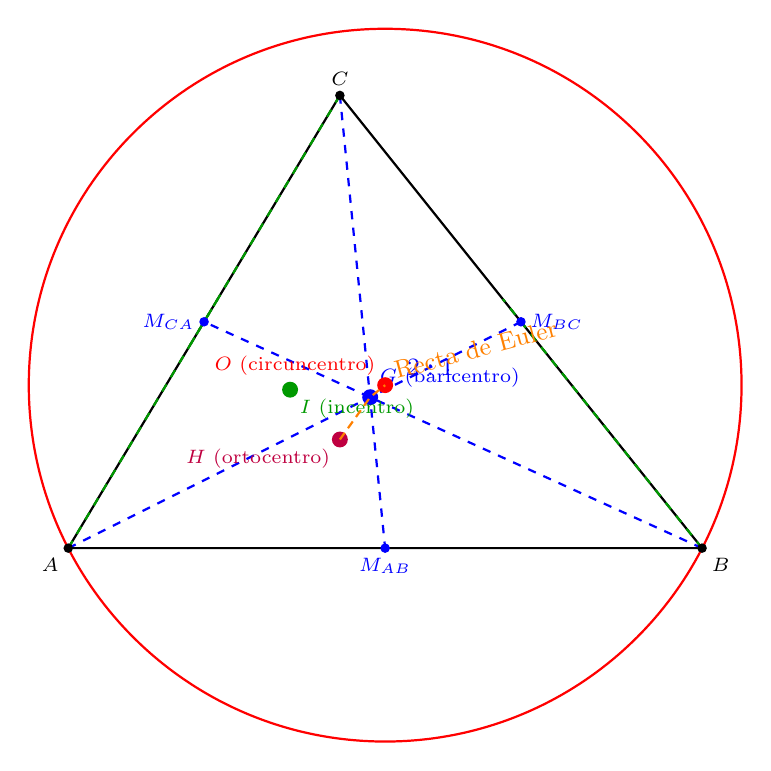
\begin{tikzpicture}[scale=1.15]

  % ---- Triángulo base ----
  \coordinate (A) at (0,0);
  \coordinate (B) at (7,0);
  \coordinate (C) at (3,5);

  \draw[thick] (A) -- (B) -- (C) -- cycle;

  % ---- Puntos medios de los lados ----
  \coordinate (M_AB) at ($(A)!0.5!(B)$);
  \coordinate (M_BC) at ($(B)!0.5!(C)$);
  \coordinate (M_CA) at ($(C)!0.5!(A)$);

  % ---- Medianas (trazadas) ----
  \draw[blue, dashed, thick] (A) -- (M_BC);
  \draw[blue, dashed, thick] (B) -- (M_CA);
  \draw[blue, dashed, thick] (C) -- (M_AB);

  % ---- Baricentro G (intersección de medianas) ----
  \coordinate (G) at ($(A)!0.667!(M_BC)$);
  \fill[blue] (G) circle (2.5pt) node[above right] {\scriptsize $G$ (baricentro)};
  \node[blue, font=\scriptsize] at ($(G)!0.4!(M_BC)$) {\small $2:1$};

  % ---- Bisectrices (trazadas, verde) ----
  \draw[green!60!black, dashed, thick] (A) -- ($(A)!0.55!(C)$);
  \draw[green!60!black, dashed, thick] (B) -- ($(B)!0.55!(C)$);
  \draw[green!60!black, dashed, thick] (C) -- ($(C)!0.55!(A)$);

  % ---- Incentro I ----
  \coordinate (I) at (2.45, 1.75);
  \fill[green!60!black] (I) circle (2.5pt) node[below right] {\scriptsize $I$ (incentro)};

  % ---- Circuncentro O ----
  \coordinate (O) at (3.5, 1.8);
  \fill[red] (O) circle (2.5pt) node[above left] {\scriptsize $O$ (circuncentro)};
  \draw[red, thick] (O) circle ({veclen(3.5,1.8)});

  % ---- Ortocentro H ----
  \coordinate (H) at (3, 1.2);
  \fill[purple] (H) circle (2.5pt) node[below left] {\scriptsize $H$ (ortocentro)};

  % ---- Etiquetas de vértices ----
  \fill (A) circle (1.5pt) node[below left] {\scriptsize $A$};
  \fill (B) circle (1.5pt) node[below right] {\scriptsize $B$};
  \fill (C) circle (1.5pt) node[above] {\scriptsize $C$};

  % ---- Puntos medios etiquetados ----
  \fill[blue] (M_AB) circle (1.5pt) node[below] {\scriptsize $M_{AB}$};
  \fill[blue] (M_BC) circle (1.5pt) node[right] {\scriptsize $M_{BC}$};
  \fill[blue] (M_CA) circle (1.5pt) node[left] {\scriptsize $M_{CA}$};

  % ---- Línea de Euler (G, O, H colineales) ----
  \draw[orange, thick, dash pattern=on 3pt off 2pt] (H) -- (G) -- (O);
  \node[orange, font=\scriptsize, rotate=15] at (4.5, 2.2) {\small Recta de Euler};

\end{tikzpicture}

\end{document}
